\documentclass{utmreport}
\newcommand{\ReportTitle}{Caesar Cipher over the Romanian Alphabet}
\newcommand{\ReportSubtitle}{\ReportCourse: standard and keyword-permuted variants}
% Load after defining ReportTitle; optional per-report settings follow below.
% Shared identity and course details for all laboratory reports.
\student{Gafenco Victor}{FAF-241}
\supervisor{asist. univ. Zaica Maia}{}
\newcommand{\ReportCourse}{Cryptography}
\cityyear{Chișinău}{2026}
\institution{Technical University of Moldova}
\faculty{Faculty of Computers, Informatics, and Microelectronics}
\department{Department of Software Engineering}
\studyprogramme{Software Engineering Study Programme}
\newcommand{\repositoryurl}{https://github.com/yoda-dinmd/crypt-labs}

\providecommand{\ReportNumber}{\expandafter\ReportNumberFromJob\jobname\relax}
\def\ReportNumberFromJob#1#2#3#4\relax{#4}
\providecommand{\ReportSubtitle}{}
\selectlanguage{english}
\ifPDFTeX\else\setmonofont{Liberation Mono}\fi
\utmlogo{../latex/assets/UTM_Logo_English.jpeg}
\documenttype{Laboratory report no. \ReportNumber}
\reporttitle{\ReportTitle}
\reportsubtitle{\ReportSubtitle}
\hypersetup{
  pdftitle={\ReportTitle},
  pdfauthor={\UTMStudentName},
  pdfsubject={\ReportCourse{} laboratory report no. \ReportNumber}
}

% Shared wording for references to the supplied Cryptography handouts.
% Arguments: laboratory number, topic, optional descriptive text (including punctuation).
\newcommand{\ReportHandoutReference}[3]{%
  \textit{Laboratory Work No. #1. #2}. Supplied course handout#3}

\lstset{language=Java}
\begin{document}
\makeutmreporttitlepage
\tableofcontents
\clearpage
\begin{utmabstract}[Abstract]
This laboratory implements the Caesar cipher and its keyword-based extension in Java for the 31-letter Romanian alphabet. Both variants use explicit alphabet positions, accept shifts from 1 to 30, and provide encryption and decryption through an interactive console. The implementation validates text and keys, normalizes case and Romanian diacritics, and prints the keyword permutation. Console captures demonstrate successful round trips and recovery from invalid input. Automated tests cover every letter and permitted shift. The experiment illustrates the weakness of a small key space and the remaining frequency-analysis vulnerability of a monoalphabetic substitution.
\utmkeywords{Caesar cipher, Romanian alphabet, permutation, Java, input validation}
\end{utmabstract}
\utmintroduction
The objective is to implement Tasks 1.1 and 1.2 of the supplied laboratory handout \cite{handout}, using its Romanian letter encoding rather than ASCII or Unicode character values for shifts. A Maven parent project contains the \texttt{lab1} module, allowing later laboratories to be added independently. Java 17 is the minimum supported version.

\chapter{Short theory}
\section{Standard Caesar cipher}
The alphabet contains $n=31$ letters, in the following order:
\begin{center}
\texttt{AĂÂBCDEFGHIÎJKLMNOPQRSȘTȚUVWXYZ}.
\end{center}
The positions are $A=0$, $\text{Ă}=1$, $\text{Â}=2$, through $Z=30$. For $k\in\{1,\ldots,30\}$, encryption and decryption are:
\begin{equation} c=(x+k)\bmod31,\qquad m=(y-k)\bmod31.\end{equation}
Here $x$ and $y$ are positions in the active alphabet. The standard cipher has 30 possible keys and can be attacked by trying every shift. Uppercasing and space removal mean decryption recovers the normalized plaintext, not its original formatting.

\section{Keyword permutation}
A keyword of at least seven Romanian letters determines a new alphabet. Its distinct letters are written in their first-occurrence order; unused letters follow in their natural order. The same formulas then use positions in this permuted alphabet for both input and output. For \texttt{CRYPTOGRAPHY}, the Romanian permutation is:
\begin{center}\texttt{CRYPTOGAHĂÂBDEFIÎJKLMNQSȘȚUVWXZ}.\end{center}
Keyword length is checked before duplicate removal, so a seven-letter keyword with repeated letters is valid. Because arbitrary sequences are permitted, all $31!$ permutations are attainable. The nominal permutation--shift key space is $30\cdot31!\approx2.47\cdot10^{35}$, but different pairs can produce the same substitution. In fact, conjugating a nonzero shift modulo the prime 31 yields a single 31-cycle, so this construction has $30!$ distinct substitutions. The larger nominal key space does not eliminate frequency analysis: a letter always maps to the same letter \cite{handout}.

\chapter{Implementation}
\section{Letter encoding and normalization}
The constant \texttt{ALPHABET} stores exactly the handout's order. Lookup with \texttt{indexOf} obtains a position; \texttt{charAt} retrieves a letter. Unicode is used to represent and normalize letters, never to calculate the cipher shift. NFC normalization accepts decomposed diacritics; cedilla forms Ş and Ţ are mapped to Ș and Ț. Only ordinary spaces are removed from messages; keywords cannot contain spaces. Blank messages are rejected to keep the console interaction meaningful.
\begin{lstlisting}
String composed = Normalizer.normalize(text, Normalizer.Form.NFC);
String letter = original.toUpperCase(Locale.ROOT)
        .replace('Ş', 'Ș').replace('Ţ', 'Ț');
String allowed = ALPHABET + ALPHABET.toLowerCase(Locale.ROOT) + "ŞşŢţ";
if (allowed.indexOf(original) < 0 || letter.length() != 1
        || ALPHABET.indexOf(letter.charAt(0)) < 0) {
    throw new IllegalArgumentException("Rejected character ...");
}
\end{lstlisting}
Each original code point is validated separately before concatenation. This prevents a non-Romanian character such as the German sharp s from being accepted through an uppercase expansion to two valid letters. Errors identify the rejected character and allowed alphabet.

\section{Building the permutation}
\begin{lstlisting}
String normalized = normalize(keyword, false);
if (normalized.length() < 7) {
    throw new IllegalArgumentException("Keyword must contain at least 7 Romanian letters; spaces are not allowed.");
}
StringBuilder permutation = new StringBuilder();
for (char letter : (normalized + ALPHABET).toCharArray()) {
    if (permutation.indexOf(String.valueOf(letter)) < 0) {
        permutation.append(letter);
    }
}
\end{lstlisting}
The first occurrence of each letter is appended once. Iterating over the keyword followed by the natural alphabet guarantees all 31 letters appear. The console prints the completed permutation before processing the message.

\section{Encryption and decryption}
\begin{lstlisting}
validateKey(key);
String normalized = normalize(text, true);
StringBuilder result = new StringBuilder();
for (char letter : normalized.toCharArray()) {
    int position = alphabet.indexOf(letter);
    int shifted = Math.floorMod(position + (decrypt ? -key : key),
                                alphabet.length());
    result.append(alphabet.charAt(shifted));
}
\end{lstlisting}
Both operations share one implementation; only the direction differs. \texttt{Math.floorMod} handles negative subtraction and wraparound. The numeric key is validated before transformation.

\section{Input validation and project structure}
The console asks for the variant, operation, numeric key, optional keyword, and message. It retries the same field after an invalid entry. A generic input helper catches validation exceptions:
\begin{lstlisting}
while (true) {
    System.out.print(prompt);
    if (!input.hasNextLine()) { return null; }
    try {
        return parser.apply(input.nextLine());
    } catch (IllegalArgumentException exception) {
        System.out.println("Invalid input: " + exception.getMessage());
    }
}
\end{lstlisting}
End of input terminates cleanly. The menu supports repeated operations and exit with zero. The root Maven POM aggregates \texttt{lab1}; the module builds an executable JAR. JUnit is a test dependency only, and the application has no external runtime dependencies.

\chapter{Results}
\section{Encryption and decryption}
The images below render actual console sessions captured from the executable Java program through a pseudo-terminal, including echoed input. They can be regenerated using the capture script in the repository; adjacent text files preserve the raw transcripts. These are reproducible console captures, rather than desktop screenshots.

Figure \ref{fig:standard} demonstrates standard encryption with $k=3$ and subsequent decryption. The normalized message \texttt{CIFRULCEZAR} becomes \texttt{FKITXOFHÂBT}. The handout's English example uses a different alphabet and therefore gives a different ciphertext.
\begin{figure}[htbp]
\centering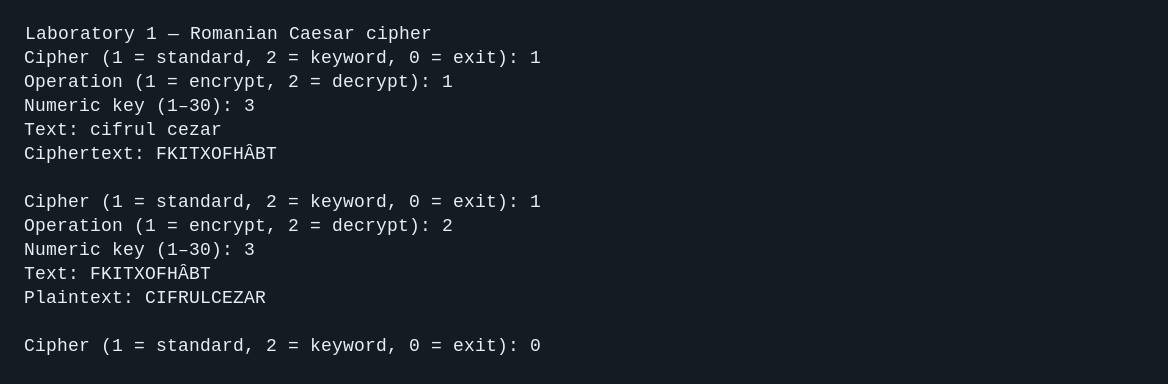
\includegraphics[width=\textwidth]{screenshots/standard.png}
\caption{Standard Romanian Caesar encryption and decryption}\label{fig:standard}
\end{figure}

Figure \ref{fig:keyword} uses keyword \texttt{CRYPTOGRAPHY} and $k=3$. The ciphertext is \texttt{PKJTXQPÎYÂT}; decryption with the same two keys recovers \texttt{CIFRULCEZAR}.
\begin{figure}[htbp]
\centering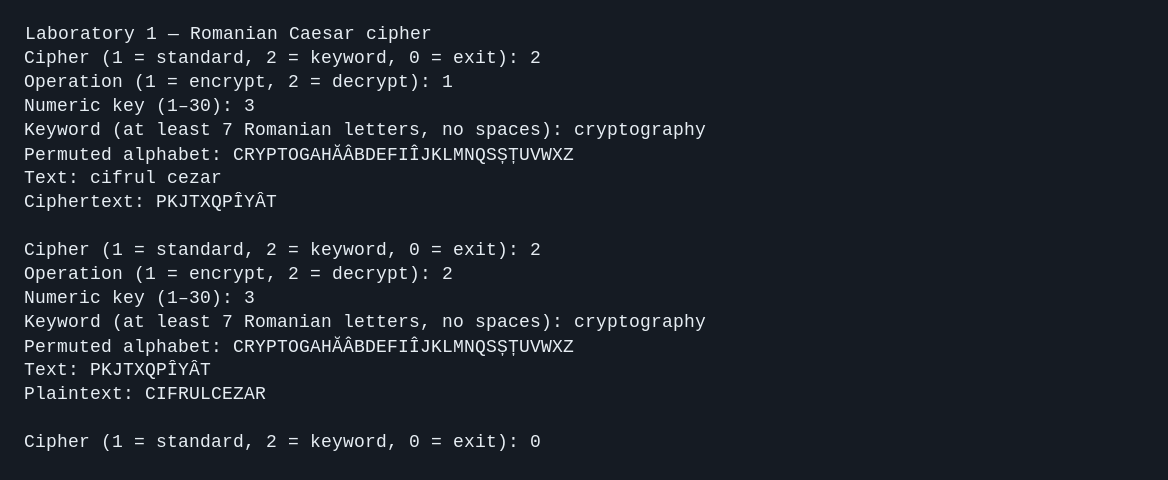
\includegraphics[width=\textwidth]{screenshots/keyword.png}
\caption{Keyword permutation, encryption and decryption}\label{fig:keyword}
\end{figure}
\clearpage
\section{Invalid input}
Figure \ref{fig:invalid} shows rejection of zero, 31, and a noninteger numeric key, a six-letter keyword, a keyword containing a space, and a message containing an exclamation mark. Each rejected field is requested again. The corrected inputs complete encryption successfully.
\begin{figure}[htbp]
\centering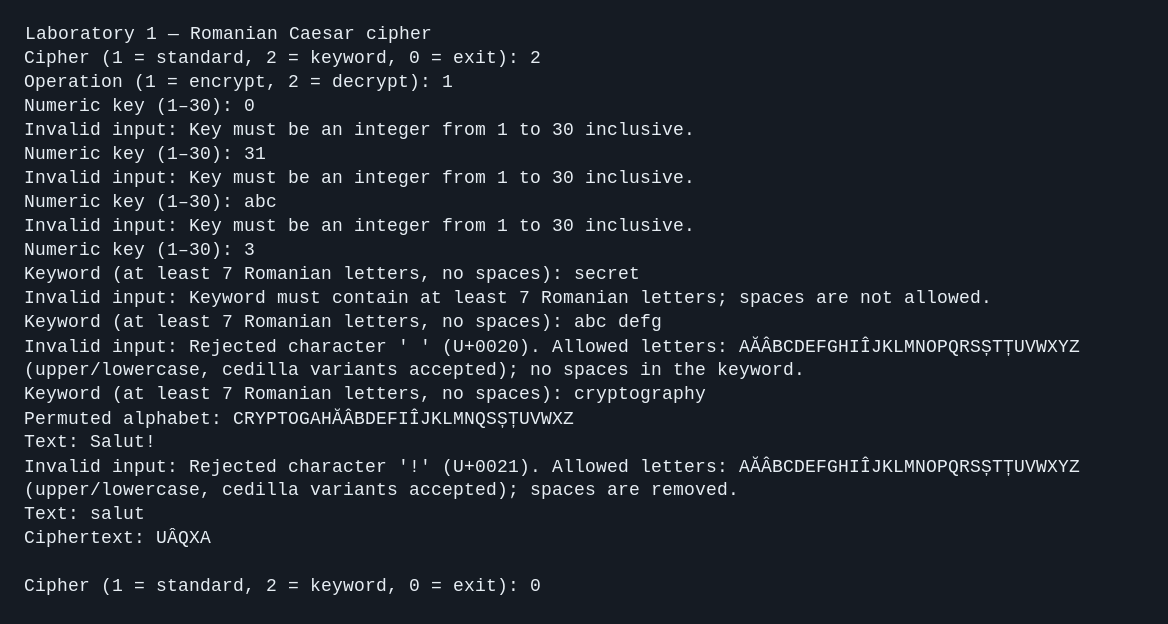
\includegraphics[width=\textwidth]{screenshots/invalid.png}
\caption{Validation messages and successful recovery}\label{fig:invalid}
\end{figure}

\section{Automated verification}
Five JUnit tests check the exact alphabet, wraparound, known Romanian ciphertexts, the exact keyword permutation, case and space normalization, cedilla and decomposed diacritics, invalid numeric keys, forbidden characters and invalid keywords. The round-trip test covers every alphabet letter at all 30 shifts for both the natural alphabet and a keyword permutation, giving 60 full-alphabet round trips. The Maven \texttt{package} lifecycle runs these tests and builds the executable JAR.

\utmconclusions
The implementation demonstrates explicit Romanian letter encoding, modular arithmetic and the construction of a keyword-derived permutation. Encryption and decryption recover the normalized input for both tasks, while validation prevents malformed keys and unsupported characters from reaching the transformation. The standard cipher is insecure because only 30 shifts need to be tried. The keyword variant increases the possible substitutions but remains monoalphabetic and exposes repeated-letter patterns and language frequencies. Neither variant is appropriate for protecting real confidential data.

\chapter*{Source code}
\addcontentsline{toc}{chapter}{Source code}
The full Java source, Maven configuration, tests and report sources are maintained in the laboratory repository: \url{\repositoryurl}.
\begin{thebibliography}{9}
\bibitem{handout} \ReportHandoutReference{1}{Caesar Cipher}{, Tasks 1.1 and 1.2 and report requirements, pp. 1--4.}
\end{thebibliography}
\end{document}
